\documentclass{beamer}

\usepackage{graphicx}
\graphicspath{ {./images/} }
\setbeamertemplate{navigation symbols}{}

\title{Anomaly Detection}
\author{Davin Ahn}
\date{November 04, 2022}

\begin{document}
    \begin{frame}
        \titlepage
    \end{frame}

    \begin{frame}
        \frametitle{Inhalt}
        \begin{enumerate}
            \item Ausreißererkennung durch Isolation Forest
            \begin{enumerate}
                \item{Hyperparameter einsetzen}
                \item{Trainierung}
                \item{Visualisieren}
                \item{Resultat}
            \end{enumerate}

            \item Model Trainieren mit anomalen erkannten Daten
            \begin{enumerate}
                \item{Resultat}
                \item{Analyse}
            \end{enumerate}
        \end{enumerate}
    \end{frame}

    \begin{frame}
        \frametitle{Ausreißererkennung durch Isolation Forest}
        \framesubtitle{Hyperparameter einsetzen}
        \centering
        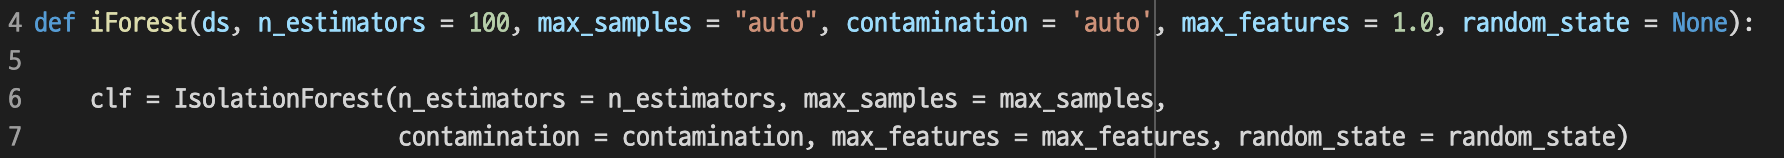
\includegraphics[scale=0.35]{parameter1.png}
        
\includegraphics[scale=0.54]{parameter2.png}
    \end{frame}

    \begin{frame}
        \frametitle{Ausreißererkennung durch Isolation Forest}
        \framesubtitle{Hyperparameter einsetzen}
        \centering
        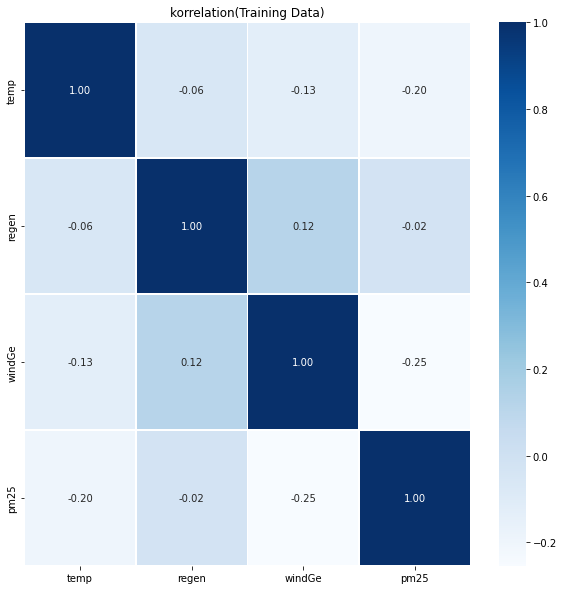
\includegraphics[scale=0.37]{korrelation.png}
    \end{frame}
    
    \begin{frame}
        \frametitle{Ausreißererkennung durch Isolation Forest}
        \framesubtitle{Trainierung}
        \centering
        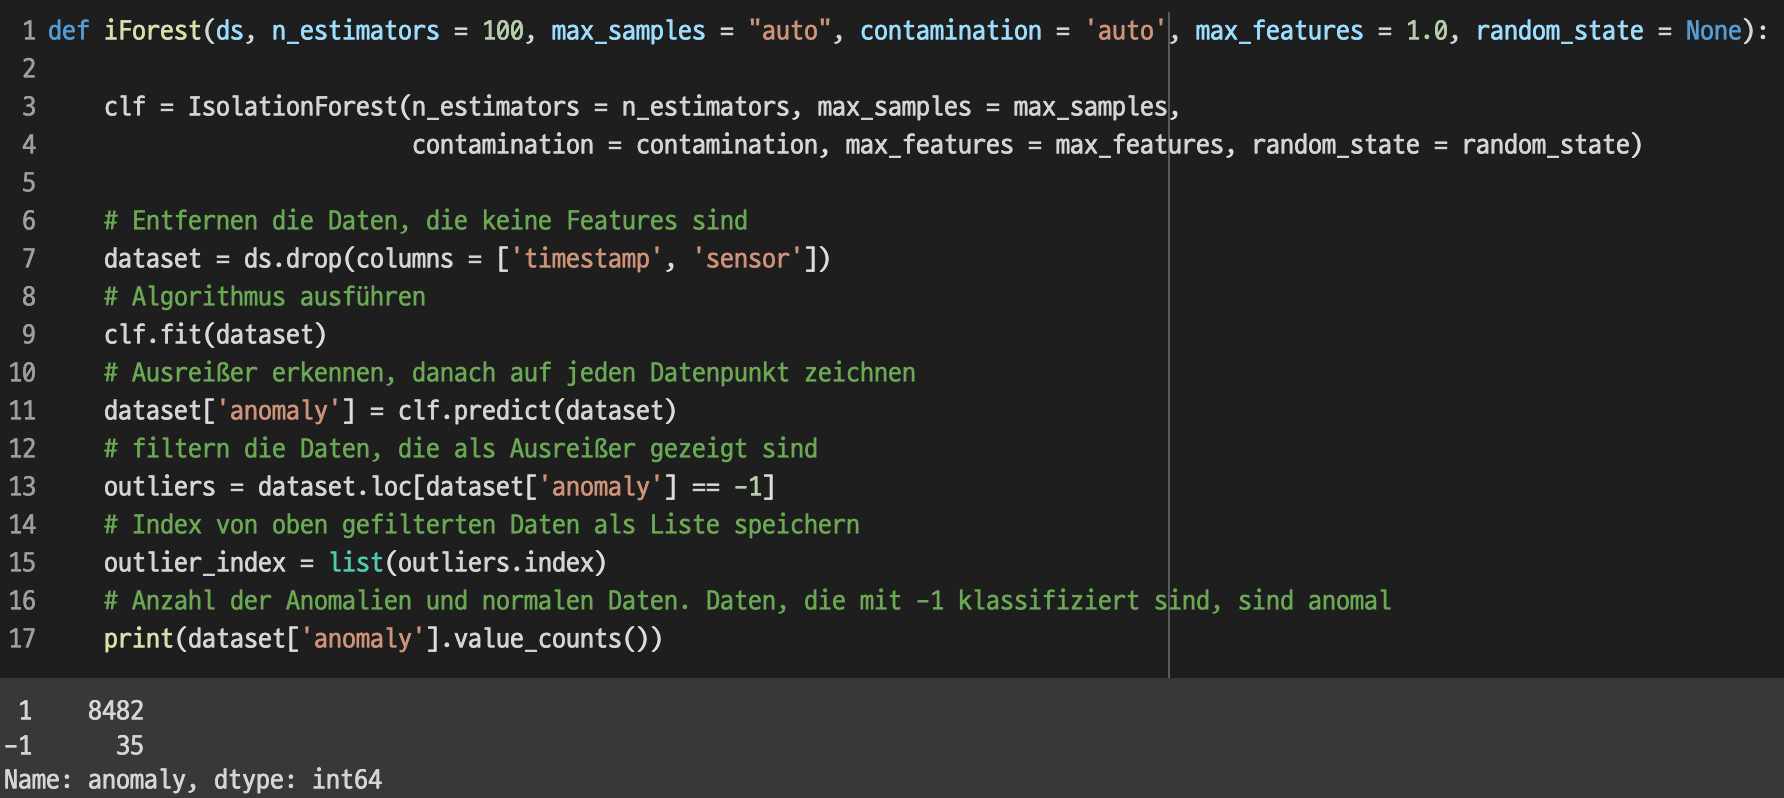
\includegraphics[scale=0.35]{training.png}
    \end{frame}
    
    \begin{frame}
        \frametitle{Ausreißererkennung durch Isolation Forest}
        \centering
        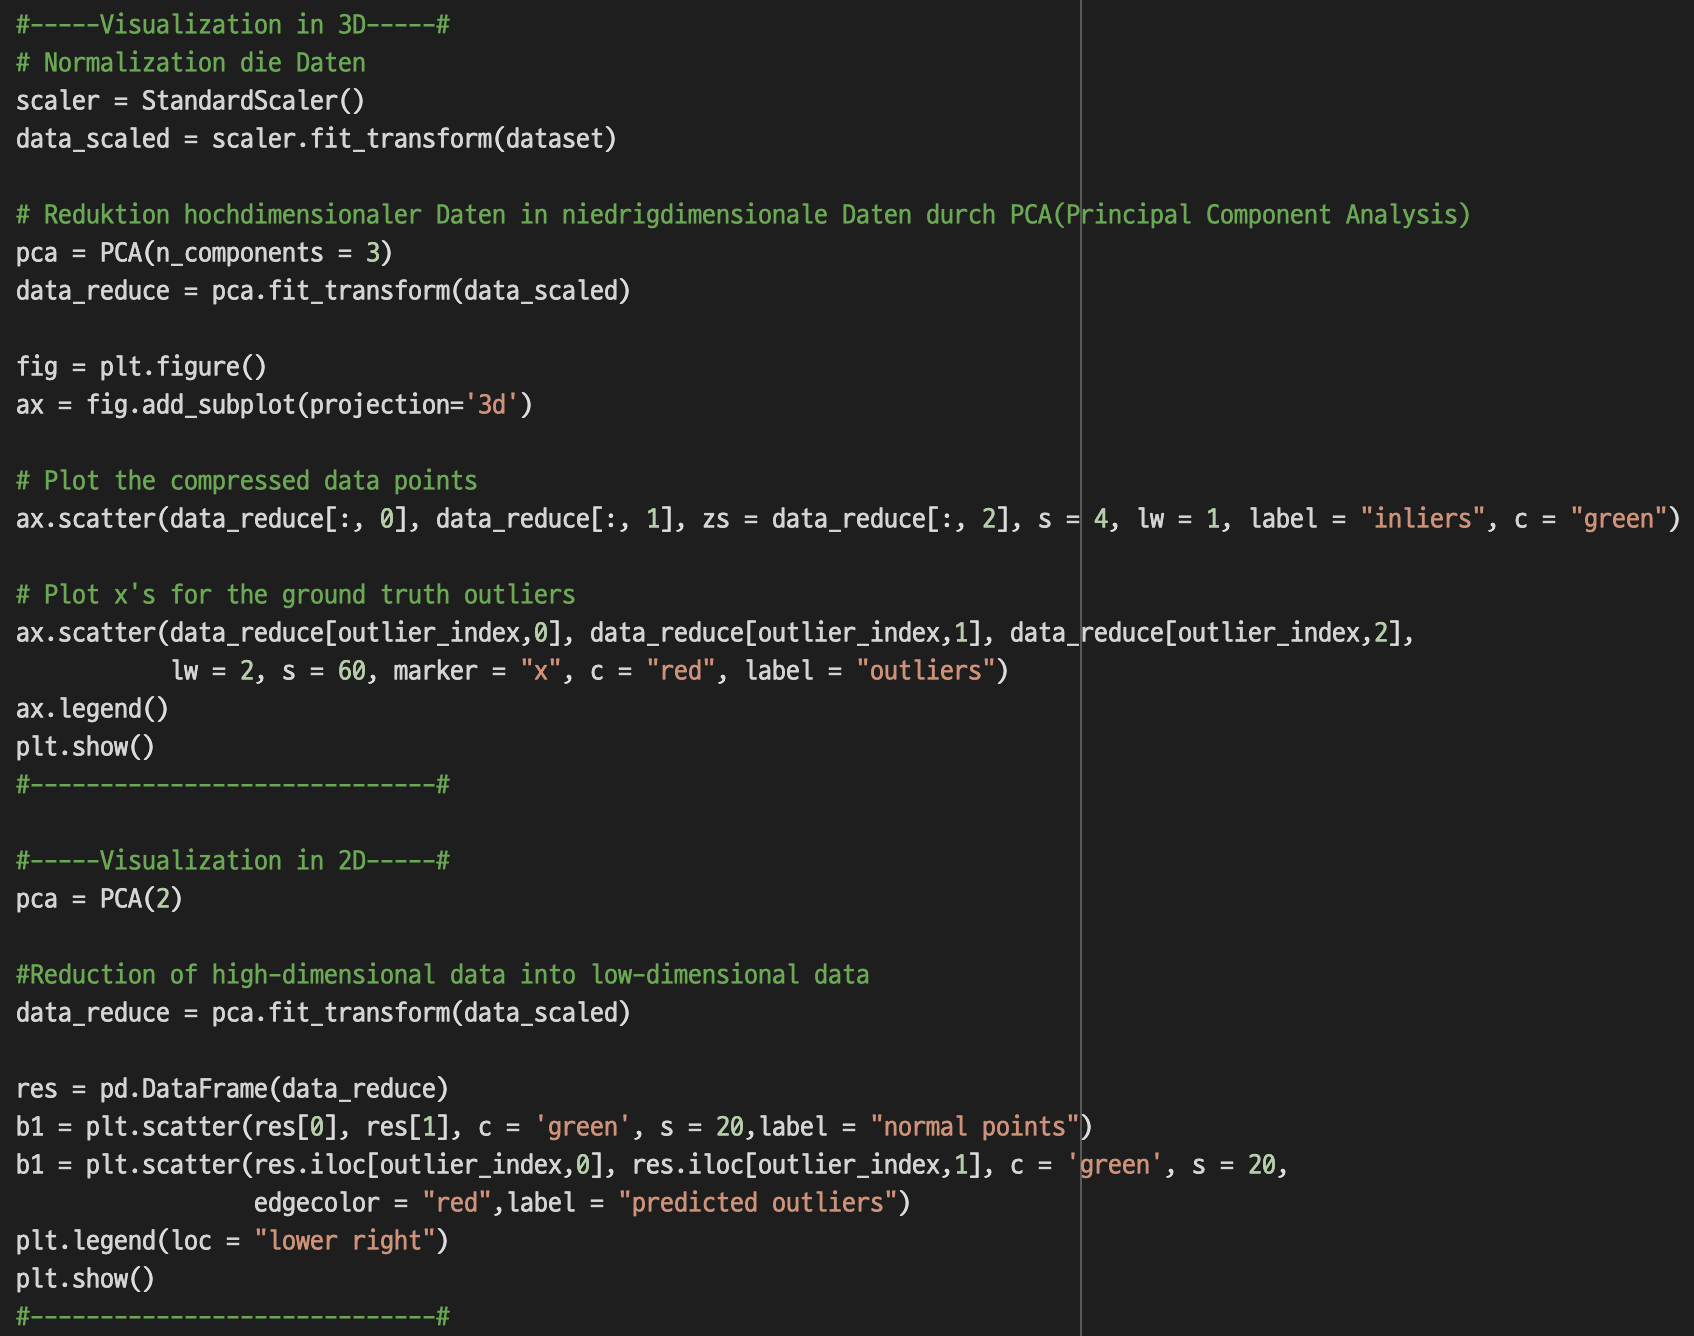
\includegraphics[scale=0.35]{visualisieren.png}
    \end{frame}
    
    \begin{frame}
        \frametitle{Ausreißererkennung durch Isolation Forest}
        \centering
        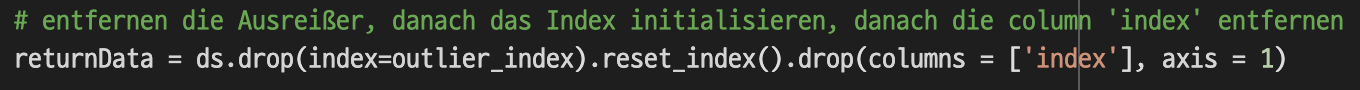
\includegraphics[scale=0.45]{weiterverarbeiten.png}
    \end{frame}
    
    \begin{frame}
        \frametitle{Ausreißererkennung durch Isolation Forest}
        \framesubtitle{Resultat}
        
        \begin{figure}[ht]
            \centering
            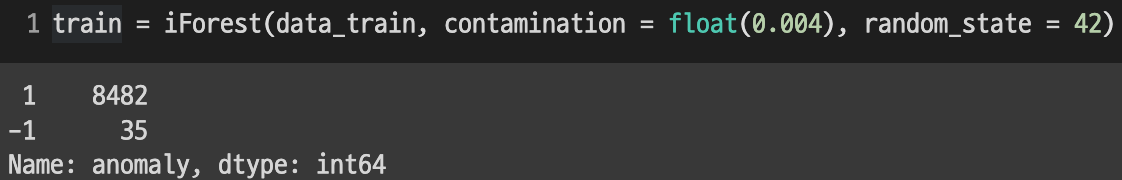
\includegraphics[scale=0.5]{Resultat1.png}
            \hfil
        
            \subfloat{
                \begin{minipage}[c][1\width]{
                0.45\textwidth}
                \centering
                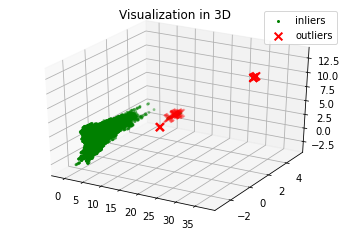
\includegraphics[width=1\textwidth]{Resultat2.png}
                \end{minipage}}
            \hfill 	
            \subfloat{
                \begin{minipage}[c][1\width]{
                0.45\textwidth}
                \centering
                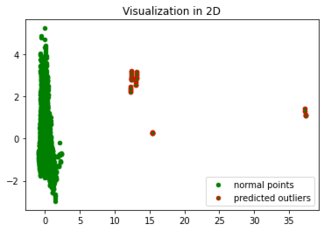
\includegraphics[width=1.1\textwidth]{Resultat3.png}
                \end{minipage}}
            \hfill
         
        \end{figure}
    \end{frame}
    
    \begin{frame}
        \frametitle{Ausreißererkennung durch Isolation Forest}
        \framesubtitle{Resultat}
        
        \begin{figure}[ht]
            \centering
            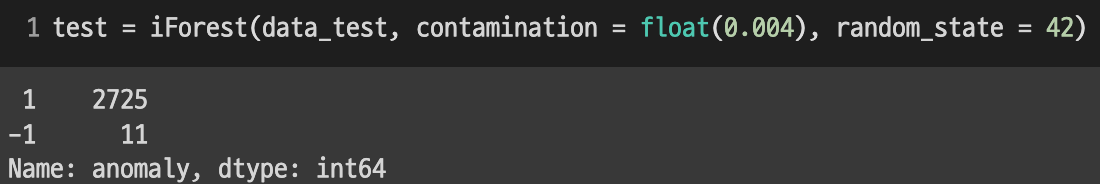
\includegraphics[scale=0.5]{Resultat4.png}
            \hfil
        
            \subfloat{
                \begin{minipage}[c][1\width]{
                0.45\textwidth}
                \centering
                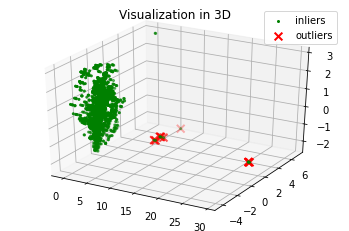
\includegraphics[width=1\textwidth]{Resultat5.png}
                \end{minipage}}
            \hfill 	
            \subfloat{
                \begin{minipage}[c][1\width]{
                0.45\textwidth}
                \centering
                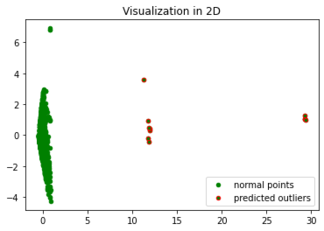
\includegraphics[width=1.1\textwidth]{Resultat6.png}
                \end{minipage}}
            \hfill
         
        \end{figure}
    \end{frame}
    
    
    \begin{frame}
        \frametitle{Model Trainieren mit anomalen erkannten Daten}
        \framesubtitle{Resultat}
        \centering
        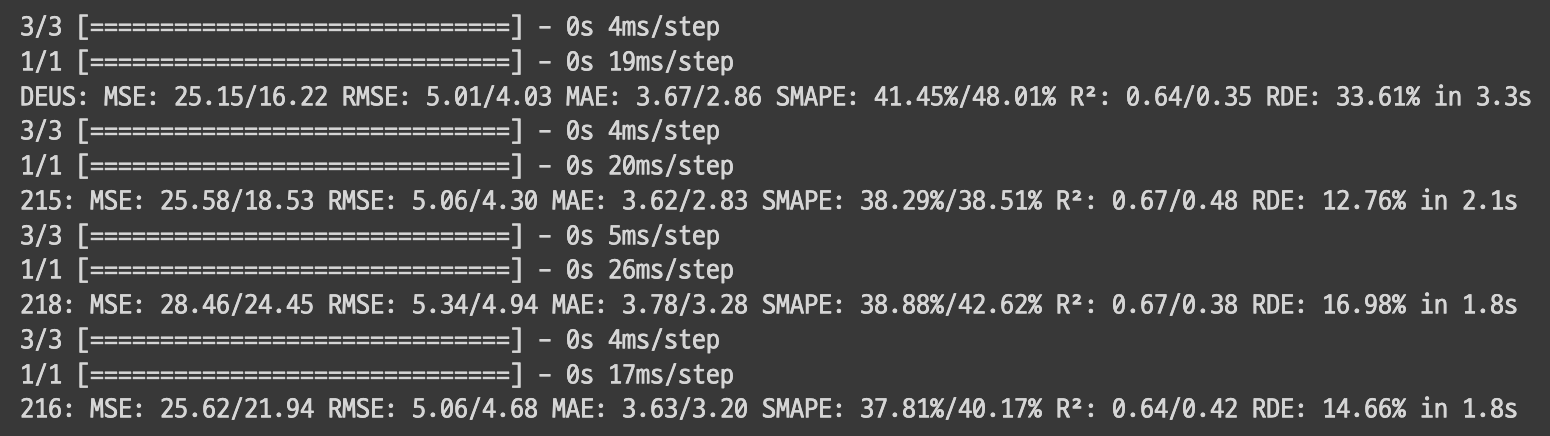
\includegraphics[scale=0.39]{prediction.png}
        \caption{Evaluation mit originalem Datensatz}
        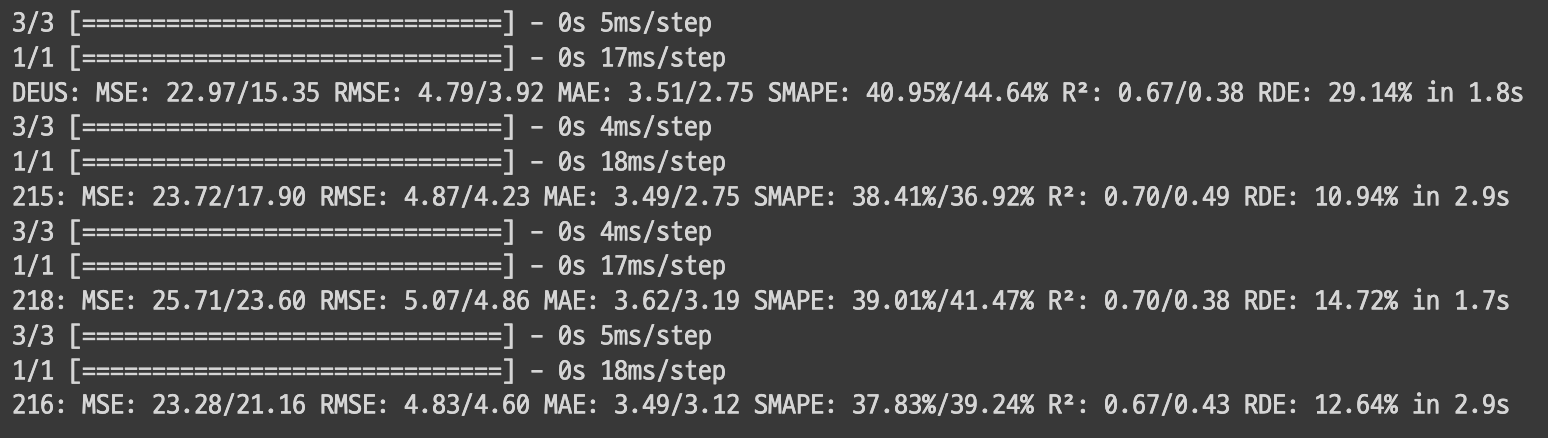
\includegraphics[scale=0.39]{prediction_re.png}
        \caption{Evaluation mit anomalien erkanntem Datensatz}
    \end{frame}

    \begin{frame}
        \frametitle{Model Trainieren mit anomalen erkannten Daten}
        \framesubtitle{Resultat}
        \centering
        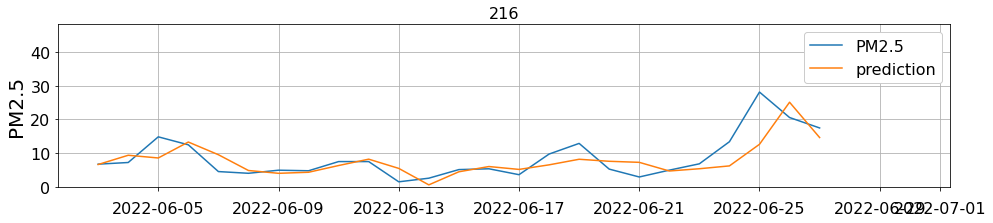
\includegraphics[scale=0.29]{216.png}
        \caption{Evaluation mit originalem Datensatz}
        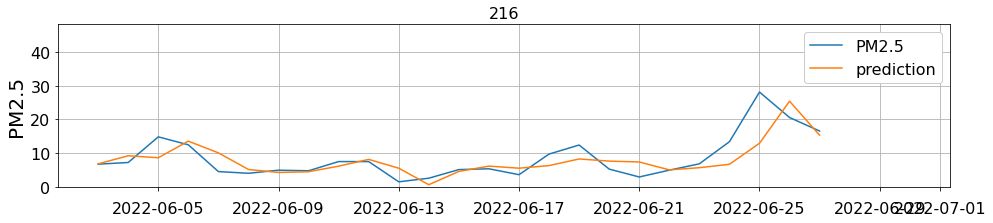
\includegraphics[scale=0.29]{216_re.png}
        \caption{Evaluation mit anomalien erkanntem Datensatz}
    \end{frame}
    
    \begin{frame}
        \frametitle{Model Trainieren mit anomalen erkannten Daten}
        \framesubtitle{Analyse}
        \centering
        %\includegraphics[scale=0.5]{Analyse.png}
    \end{frame}
    
\end{document}